% modelo_prova.tex (versão final com o novo design e toda a lógica do projeto)
\documentclass[12pt, a4paper]{article}

% --- PACOTES ---
\usepackage{fontspec}
\usepackage[brazil]{babel}
\usepackage{graphicx}
\usepackage[space]{grffile}
\usepackage{amsmath}
\usepackage[svgnames]{xcolor}
\usepackage{fancyhdr}
\usepackage{lastpage}
\usepackage{enumitem}
\usepackage{tabularx}
\usepackage{calc}
\usepackage{colortbl}
\usepackage{array}
\usepackage{geometry}
\usepackage{amsfonts}
\usepackage{amssymb}
\usepackage{ifthen}
\usepackage{tasks}

\setmainfont{Times New Roman}

% --- Geometria da Página e Cabeçalho (com ajustes do log) ---
\geometry{a4paper, top=1.5cm, bottom=1.5cm, left=2cm, right=2cm, 
    headheight=40pt, 
    includehead, includefoot}

% --- AJUSTE GLOBAL DE PARÁGRAFO ---
\setlength{\parindent}{0pt} 

% --- Configuração do Cabeçalho e Rodapé ---
\pagestyle{fancy}
\fancyhf{}

% CABEÇALHO
\fancyhead[L]{
\includegraphics[height=1.5cm]{logo-iff.png}}
\fancyhead[R]{%
    \begin{tabular}{@{}r@{}}
        \textbf{\textit{<<nomeDisciplina>>}} \\
        \textbf{\textit{CADERNO <<versao>>}}
    \end{tabular}%
}

% RODAPÉ
\fancyfoot[C]{%
    \begin{tabular}{@{}c@{}}
        \small \textit{Prof. <<nomeProfessor>>} \\
        \small \textit{<<emailContato>>} \\
        \small \textit{<<nomeescola>>}
    \end{tabular}%
}
\fancyfoot[R]{\thepage} % Número da página
\renewcommand{\headrulewidth}{0.4pt}
\renewcommand{\footrulewidth}{0.4pt}

% --- Estilo Personalizado para a Capa ---
\fancypagestyle{capa}{
    \fancyhf{}
    \fancyhead[L]{
\includegraphics[height=1.5cm]{logo-iff.png}}
    \fancyhead[R]{%
        \begin{tabular}{@{}r@{}}
            \textbf{\textit{<<nomeDisciplina>>}} \\
            \textbf{\textit{CADERNO <<versao>>}}
        \end{tabular}%
    }
    \fancyfoot[C]{%
        \begin{tabular}{@{}c@{}}
            \small \textit{Prof. <<nomeProfessor>>} \\
            \small \textit{<<emailContato>>} \\
            \small \textit{<<nomeescola>>}
        \end{tabular}%
    }
    \renewcommand{\headrulewidth}{0pt}
    \renewcommand{\footrulewidth}{0pt}
    \fancyfoot[R]{}
}

% --- Comando para o Título da Questão (Argumentos: 1=Número, 2=Valor) ---
% Unindo o design do seu novo modelo com a funcionalidade do antigo (exibir valor)
\newcommand{\questiontitle}[1]{%
    \par 
    \noindent
    \fcolorbox{gray}{lightgray}{%
        \parbox{\dimexpr\linewidth-2\fboxsep-2\fboxrule\relax}{%
            \centering
            \textbf{QUESTÃO #1}%
        }%
    }%
    \par\vspace{0.4cm}%
}

% #################### INÍCIO DO DOCUMENTO ####################
\begin{document}
    \thispagestyle{capa}
    
    % --- Tabela para os dados do Aluno (do seu novo modelo) ---
    \begin{center}
         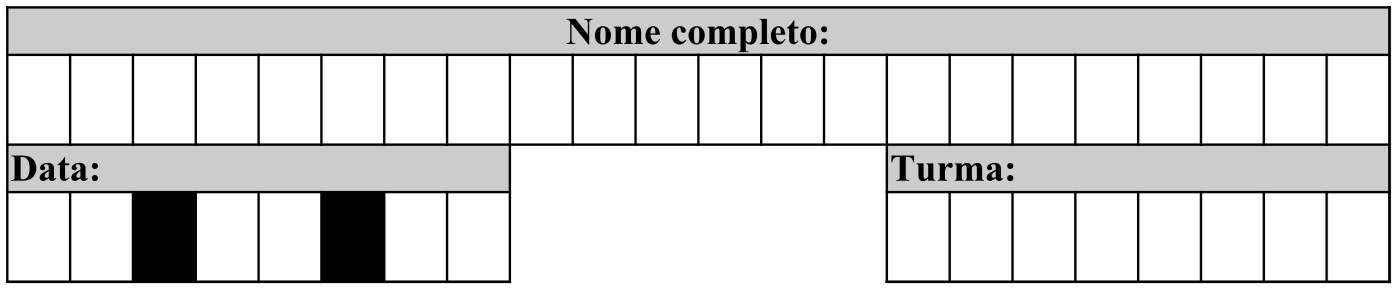
\includegraphics[width=\textwidth]{tabela_dados_aluno.png} 
    \end{center}
    
    % --- Capa da Prova (seguindo seu novo modelo, mas com variáveis) ---
    \begin{center}
        \fcolorbox{black}{black}{%
            \begin{minipage}[c][1.8cm][c]{0.6\textwidth}
                \centering \color{white}
                {\bfseries\fontsize{28}{26}\selectfont <<siglaCurso>>} \\[0.2cm]
                {\small <<nomeCursoCompleto>>}
            \end{minipage}%
        }
        
        \vspace*{0.5cm}
        
        \fcolorbox{black}{black}{%
            \begin{minipage}[c][1.5cm][c]{0.75\textwidth}
                \centering \color{white} \fontsize{28}{28}\selectfont \textbf{AVALIAÇÃO BIMESTRAL}
            \end{minipage}%
        }\fcolorbox{black}{DarkGray}{%
            \begin{minipage}[c][1.5cm][c]{0.12\textwidth}
                \centering \color{white} \fontsize{36}{40}\selectfont \textbf{<<bimestre>>}
            \end{minipage}%
        }
    \end{center}
    
    \vspace*{0.14cm}
    \noindent\fcolorbox{black}{white}{\parbox{\dimexpr\textwidth-2\fboxsep-2\fboxrule\relax}{\centering\textbf{\Large <<nomeDisciplina|upper>>}}}
    
    \vspace*{0.4cm}
    \noindent\fcolorbox{black}{lightgray}{\parbox{\dimexpr\textwidth-2\fboxsep-2\fboxrule\relax}{\centering\textbf{LEIA COM ATENÇÃO AS INSTRUÇÕES ABAIXO.}}}
    
    \begin{enumerate}[label=\bfseries\arabic*. , wide, labelwidth=!, labelindent=0pt, leftmargin=*]
        % (Mantendo as novas instruções do seu último arquivo)
        \item Você está recendo o seguinte material:
        \begin{enumerate}[label=\alph*)]
            \item 1 caderno de questões, contendo: \\
            
            \noindent % Garante que o minipage comece imediatamente
            \begin{minipage}{\linewidth}
                \par\centering 
                \begingroup 
                \setlength{\extrarowheight}{3pt} 
                \arrayrulecolor{black} 
                
                \begin{tabular}{|c|c|c|}
                    \hline
                    \rowcolor{lightgray} 
                    \textbf{Quantidade de questões} & \textbf{Valor de cada questão} & \textbf{Valor Total da Prova} \\
                    \hline
                    \rowcolor{white} 
                    <<numeroQuestoes>> & <<valorPorQuestao>> & <<valorTotalProva>> \\
                    \hline
                \end{tabular}
                \endgroup
            \end{minipage}
            \vspace{0.35cm}
            \item 1 cartão de respostas, destinado às respostas das questões de múltipla escolha.
        \end{enumerate}
        \item Verifique se este material está completo. Caso contrário, notifique imediatamente ao professor. 
        Após conferência, você deverá assinar o Cartão-Resposta no espaço próprio, utilizando caneta de cor PRETA ou AZUL.
        \item Observe no Cartão-Resposta as instruções sobre a marcação das respostas às questões de múltipla escolha (apenas uma resposta por questão).
        \item Tenha muito cuidado com o Cartão-Resposta, para não dobrar, amassar ou manchar.
        \item Esta prova é individual. São vedados o uso de qualquer comunicação e troca de material entre os presentes.
        \item Não será necessário apresentação dos cálculos para correção da avaliação, apenas a marcação no Cartão-Resposta.
        \item Não será permitido sair da sala com o caderno de questões e o cartão-resposta, devendo estes serem entregues ao término da avaliação.
    \end{enumerate}
    \vspace{0.5cm}
    \newpage
    
    % ========= CORPO DA PROVA (QUESTÕES) ===========
    <<% for questao in questoes %>>
    % --- Início da "caixa" que impede a quebra da questão ---
    \begin{minipage}{\linewidth} 
    
    % --- TÍTULO DA QUESTÃO (AGORA APARECE PARA TODOS OS FORMATOS) ---
    \questiontitle{<<loop.index>>}
    
    <<questao.enunciado>>

    <<% if questao.imagem %>>
        \par\vspace{0.1cm}
        \par\noindent\centering
        \includegraphics[width=<<questao.imagemLarguraPercentual / 100.0>>\textwidth]{<<questao.imagem>>}
        \par\vspace{0.1cm}
    <<% endif %>>

    % --- LÓGICA CONDICIONAL PARA O FORMATO DA QUESTÃO ---
    <<% if questao.formato_questao == 'Múltipla Escolha' %>>
        <<% if questao.is_multi_valor %>>
            % Layout Horizontal (com ajuste para warnings)
            {\footnotesize
            \begin{tasks}[label=\textbf{(\Alph*)}, label-width=2em, label-offset=0.8em](5)
            <<% for letra, texto in questao.alternativas.items()|sort %>>
                \task << texto >>
            <<% endfor %>>
            \end{tasks}
            }
        <<% else %>>
            % Layout Vertical
            \begin{enumerate}[label=\textbf{(\Alph*)}, wide, labelwidth=!, labelindent=0pt, leftmargin=*, topsep=0.5cm, itemsep=0.3cm]
            <<% for letra, texto in questao.alternativas.items()|sort %>>
                \item << texto >>
            <<% endfor %>>
            \end{enumerate}
        <<% endif %>>
    <<% elif questao.formato_questao == 'Verdadeiro ou Falso' %>>
        \vspace{0.5cm}
        \noindent ( \quad ) Verdadeiro \hspace{2cm} ( \quad ) Falso
    <<% elif questao.formato_questao == 'Discursiva' %>>
        \vspace{5cm}
    <<% endif %>>
    
    \vspace{1cm}
    \end{minipage} 
    % --- Fim da "caixa" ---
    <<% endfor %>>
    
\end{document}